\documentclass[11pt,a4paper]{article}

% ---------- Packages ----------
\usepackage[a4paper,margin=1in]{geometry}
\usepackage{times}
\usepackage[T1]{fontenc}
\usepackage{graphicx}
\usepackage{xcolor}
\usepackage{titlesec}
\usepackage{enumitem}
\usepackage{fancyhdr}
\usepackage{hyperref}
\usepackage{tabularx}
\usepackage{booktabs}
\usepackage{longtable}
\usepackage{caption}
\usepackage{listings}
\usepackage{multicol}
\usepackage{tikz}
\usetikzlibrary{positioning, arrows.meta, shapes.geometric, fit, backgrounds}

% ---------- Colors ----------
\definecolor{primaryblue}{RGB}{22,54,92}
\definecolor{accentteal}{RGB}{0,121,140}
\definecolor{lightgray}{RGB}{245,245,245}
\definecolor{codebg}{RGB}{247,247,250}

% ---------- Section styling ----------
\titleformat{\section}
  {\normalfont\Large\bfseries\color{primaryblue}}
  {\thesection}{0.6em}{}
\titleformat{\subsection}
  {\normalfont\large\bfseries\color{accentteal}}
  {\thesubsection}{0.6em}{}
\titleformat{\subsubsection}
  {\normalfont\normalsize\bfseries\color{black}}
  {\thesubsubsection}{0.6em}{}

% ---------- Header / Footer ----------
\pagestyle{fancy}
\fancyhf{}
\renewcommand{\headrulewidth}{0.4pt}
\fancyhead[L]{\small SCS 3311 -- Mobile Application Design \& Development}
\fancyhead[R]{\small Smart Home Monitoring \& Control System}
\fancyfoot[C]{\thepage}

% ---------- Hyperlinks ----------
\hypersetup{
  colorlinks=true,
  linkcolor=accentteal,
  urlcolor=accentteal,
  citecolor=accentteal,
  pdftitle={Smart Home Monitoring and Control System - Technical Report},
  pdfauthor={Group 00 - SCS 3311}
}

% ---------- Code listing style ----------
\lstdefinestyle{codestyle}{
  backgroundcolor=\color{codebg},
  basicstyle=\ttfamily\footnotesize,
  breaklines=true,
  frame=single,
  rulecolor=\color{gray!40},
  numbers=left,
  numberstyle=\tiny\color{gray},
  showstringspaces=false,
  captionpos=b,
}
\lstset{style=codestyle}

\newcommand{\todofill}[1]{\textcolor{black}{\textit{#1}}}

\begin{document}

% =====================================================
% TITLE PAGE
% =====================================================
\begin{titlepage}
    \centering
    \vspace*{1cm}
    {\large University of Colombo School of Computing\par}
    \vspace{0.3cm}
    {\large SCS 3311 -- Mobile Application Design and Development\par}
    \vspace{2cm}

    {\Huge\bfseries\color{primaryblue} Smart Home Monitoring \\ and Control System\par}
    \vspace{0.5cm}
    {\Large Technical Documentation Report\par}

    \vspace{2cm}
 \vspace{2cm}
    \begin{tabular}{ll}
        \toprule
        \textbf{Name} & \textbf{Index No.} \\
        \midrule
        R.K.K. Jinendra & 23000821 \\
        G.C.K.S. Gajanayake & 23000481 \\
        S.S. Balahewa & 23000155 \\
        \bottomrule
    \end{tabular}

\end{titlepage}

\tableofcontents
\newpage

% =====================================================
\section{Introduction}

\subsection{Project Overview}
The \textbf{Smart Home Monitoring and Control System} is a mobile-first Internet of Things (IoT) application that allows a household to monitor and control heterogeneous electrical devices distributed across multiple floor plans, from a single mobile client. The system is composed of three cooperating components:

\begin{enumerate}[label=(\roman*)]
    \item An \textbf{Android mobile application} (built with Kotlin and Jetpack Compose) that presents an interactive, multi-floor dashboard for viewing and controlling devices.
    \item A \textbf{cloud backend} (Firebase Realtime Database) that acts as the single source of truth for device state and enables low-latency bidirectional synchronization between the mobile client and the physical/simulated hardware.
    \item A \textbf{React-based web dashboard and Cloud Functions layer}, which together (a) emulate the physical appliances that would otherwise require real IoT hardware, and (b) continuously enforce server-side safety rules -- most importantly, automatically switching off fire-hazard-prone devices such as electric irons if they exceed a configured maximum active duration.
\end{enumerate}

This separation of concerns mirrors real commercial smart-home platforms (e.g. Google Home, Tuya, SmartThings), where a thin, reactive mobile client is backed by a always-on cloud service that both persists state and independently enforces safety invariants, regardless of whether the mobile app is open.

\subsection{Objectives}
\begin{itemize}
    \item Provide a single mobile interface for monitoring and controlling multiple categories of home devices across multiple floors.
    \item Guarantee near real-time, bidirectional state synchronization between the app, the cloud database, and the (simulated) physical devices.
    \item Enforce automated, backend-driven safety cut-offs for hazardous appliances, independent of client connectivity.
    \item Provide historical usage reporting for key devices.
    \item Demonstrate the end-to-end system using a React-based hardware simulator dashboard in place of physical IoT components.
\end{itemize}

\newpage
% =====================================================
\section{System Architecture}

\subsection{High-Level Architecture}
The system follows a \textbf{cloud-mediated, reactive architecture}: neither the mobile app nor the hardware simulator communicate with each other directly. Instead, both are independent listeners on a shared Firebase Realtime Database instance, and all state changes are propagated through the database. This decouples the client and the device layer completely and allows either side to be extended, replaced, or scaled independently.

\begin{figure}[h!]
\centering
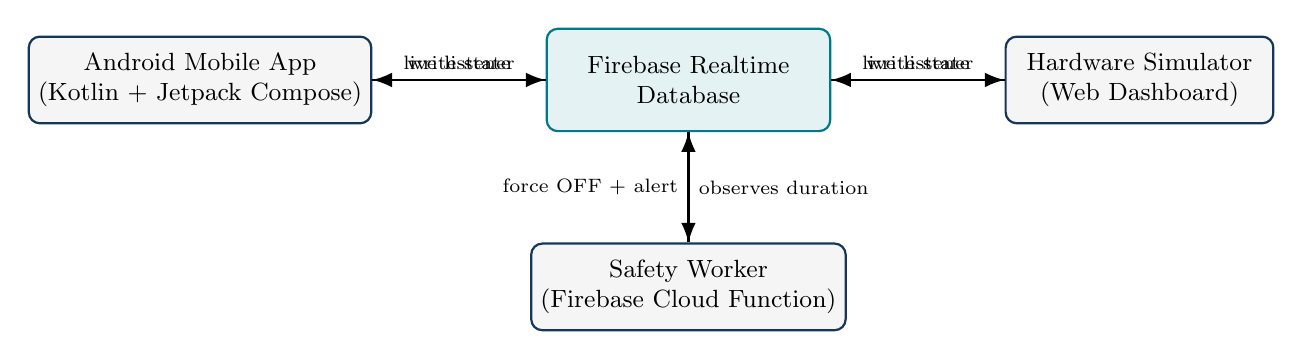
\begin{tikzpicture}[
    node distance=1.4cm and 2.2cm,
    box/.style={rectangle, rounded corners, draw=primaryblue, thick, fill=lightgray, minimum width=3.4cm, minimum height=1.1cm, align=center, font=\small},
    cloudbox/.style={rectangle, rounded corners, draw=accentteal, thick, fill=accentteal!10, minimum width=3.6cm, minimum height=1.3cm, align=center, font=\small},
    arrow/.style={-{Latex[length=2.5mm]}, thick}
]
    \node[box] (app) {Android Mobile App\\ (Kotlin + Jetpack Compose)};
    \node[cloudbox, right=of app] (fb) {Firebase Realtime\\ Database};
    \node[box, right=of fb] (sim) {Hardware Simulator\\ (Web Dashboard)};
    \node[box, below=of fb] (worker) {Safety Worker\\ (Firebase Cloud Function)};

    \draw[arrow] (app) -- node[above, font=\scriptsize]{write state} (fb);
    \draw[arrow] (fb) -- node[above, font=\scriptsize]{live listener} (app);
    \draw[arrow] (sim) -- node[above, font=\scriptsize]{write state} (fb);
    \draw[arrow] (fb) -- node[above, font=\scriptsize]{live listener} (sim);
    \draw[arrow] (fb) -- node[right, font=\scriptsize]{observes duration} (worker);
    \draw[arrow] (worker) -- node[left, font=\scriptsize]{force OFF + alert} (fb);
\end{tikzpicture}
\caption{High-level system architecture. All components communicate exclusively through the Firebase Realtime Database, which acts as the single source of truth.}
\end{figure}

\subsection{Component Responsibilities}
\begin{itemize}
    \item \textbf{Mobile Application} -- renders floor plans, device grids, and control widgets; attaches real-time listeners to the database; writes user-initiated state changes; displays alerts and usage reports.
    \item \textbf{Firebase Realtime Database} -- stores the canonical state of every floor, room, device, schedule, and usage log entry; pushes incremental updates to every connected listener with sub-second latency.
    \item \textbf{Safety Worker} -- a scheduled Firebase Cloud Function (Node.js/JavaScript) that watches all devices flagged as safety-critical (e.g. irons), tracks their \texttt{max\_on\_duration}, and force-switches them off with a database write and alert flag if the limit is breached, independent of whether a mobile client is connected.
    \item \textbf{React Hardware Simulator Dashboard} -- a browser-based visualization built with React that subscribes to the same database and mimics how the physical appliances would visually respond (LEDs, ON/OFF indicators, mock camera feed) to state changes, standing in for real hardware.
\end{itemize}

\subsection{Data Model}
The database is organized hierarchically to make partial, incremental synchronization efficient -- clients only need to attach listeners to the sub-trees they are currently displaying, rather than downloading the entire home state.

\begin{lstlisting}[language=, caption={Simplified Firebase Realtime Database structure (JSON tree)}]
smart_home/
  floors/
    floor_1/
      name: "Ground Floor"
      grid_rows: 6
      grid_cols: 8
      plan_image_url: "..."
      rooms/
        living_room/
          grid_x: 2
          grid_y: 3
          devices: [outlet_01, camera_01]
  devices/
    outlet_01/
      type: "outlet"
      floor_id: "floor_1"
      room_id: "living_room"
      status: "ON"          // ON | OFF | ERROR | DISCONNECTED
      last_updated: <timestamp>
    switchbox_01/
      type: "multi_switch"
      switch_count: 3
      switches:
        s1: { label: "Ceiling Light", status: "ON" }
        s2: { label: "Fan",           status: "OFF" }
        s3: { label: "Wall Light",    status: "OFF" }
    iron_01/
      type: "scheduled_safety"
      status: "ON"
      max_on_duration_min: 30
      turned_on_at: <timestamp>
      auto_cutoff_triggered: false
    bulb_hallway/
      type: "scheduled_lighting"
      status: "OFF"
      schedule: { start: "18:30", end: "23:00" }
    camera_01/
      type: "camera"
      stream_uri: "mock://camera_01/snapshot"
      status: "ON"
  usage_logs/
    outlet_01/
      2026-08-14T20:15:00Z: { action: "ON",  by: "user" }
      2026-08-14T22:40:00Z: { action: "OFF", by: "user" }
  alerts/
    <alert_id>/
      device_id: "iron_01"
      type: "AUTO_CUTOFF"
      timestamp: <timestamp>
      message: "Iron exceeded max on-duration of 30 min and was switched off automatically."
\end{lstlisting}

\newpage

% =====================================================
\section{Device Models and Control UI}

Each device category in the system was modelled as its own data schema and its own Compose UI component, to reflect the heterogeneous nature of real smart-home hardware.

\subsection{Electrical Outlets}
The simplest device type: a single binary node representing a continuous power supply to a plugged-in appliance. Exposes a single toggle control and one of the four canonical states (\texttt{ON}, \texttt{OFF}, \texttt{ERROR}, \texttt{DISCONNECTED}).

\subsection{Multi-Switch Units}
Represents a single physical gang-box (wall switch plate) that may host a variable number ($n \in \{2, 3, 5\}$) of independently addressable switches -- for example, a 3-gang switch controlling a ceiling light, a fan, and a wall light from one physical unit. In the data model this is a single device entity with a nested \texttt{switches} map, and the UI renders it as one card containing $n$ individual toggle rows, so the abstraction visible to the user matches the physical unit while still allowing independent control of each switch.

\subsection{Scheduling for Safety-Critical Devices}
Appliances that pose a fire risk if left on unattended (irons, heaters) are modelled with an additional \texttt{max\_on\_duration\_min} field. When such a device is switched ON, a \texttt{turned\_on\_at} timestamp is recorded. This value is the input used by the server-side Safety Worker Cloud Function (Section~5) to enforce an automatic cut-off.

\subsection{Scheduled Lighting}
Certain lighting devices support a preset daily \texttt{schedule} (start / end time). Rather than requiring manual toggling every day, these devices can be configured to turn on and off automatically at the configured times.

\subsection{Security Cameras}
Camera devices expose a mock snapshot URI / streaming URI rather than a real video feed (since no physical camera hardware is available for this project). The mobile UI renders these as a card showing the latest mock snapshot image and a status indicator, standing in for what would be a live video/RTSP stream in a production system.

\subsection{Unified Status Model}
All device types, regardless of category, expose the same four-state status enumeration so that the dashboard can present a consistent visual language across a heterogeneous device fleet:

\begin{table}[h!]
\centering
\begin{tabularx}{\textwidth}{lX}
\toprule
\textbf{Status} & \textbf{Meaning} \\
\midrule
\texttt{ON} & Device is actively powered / operating. \\
\texttt{OFF} & Device is intentionally powered down. \\
\texttt{ERROR} & Device reported a fault state (e.g. simulated hardware fault). \\
\texttt{DISCONNECTED} & Device has not reported a heartbeat / state update within the expected interval, and is treated as unreachable. \\
\bottomrule
\end{tabularx}
\caption{Canonical device status values used across all device types}
\end{table}

\newpage
% =====================================================
\section{Online Synchronization Mechanism}

\subsection{Bidirectional Real-Time Sync}
The system's responsiveness depends entirely on Firebase Realtime Database's listener-based synchronization model:

\begin{itemize}
    \item \textbf{Mobile $\rightarrow$ Cloud:} When a user taps a device toggle, the app immediately writes the new state to the corresponding \texttt{devices/\{id\}/status} path. Jetpack Compose's \texttt{StateFlow}-backed \texttt{ViewModel} optimistically updates the local UI state while the write is in flight, giving the user instant visual feedback.
    \item \textbf{Cloud $\rightarrow$ Mobile:} The app attaches a \texttt{ValueEventListener} (or, in Compose, a \texttt{callbackFlow}-wrapped listener collected via \texttt{collectAsState()}) to each floor/device sub-tree currently visible on screen. Any external change -- whether from another user's phone, the hardware simulator, or the safety worker -- is pushed to the client automatically, without the user needing to pull-to-refresh.
    \item \textbf{Cloud $\rightarrow$ Simulator:} The hardware simulator dashboard uses the Firebase JavaScript SDK's \texttt{onValue()} listener to mirror the same state changes visually, simulating how a physical device would respond to a remote command.
\end{itemize}

\subsection{Why Firebase Realtime Database}
Firebase Realtime Database was selected over a conventional REST + polling architecture because:
\begin{enumerate}
    \item It natively supports persistent WebSocket-based listeners, giving sub-second propagation latency with minimal client-side code.
    \item Its JSON-tree structure maps naturally onto the floor $\rightarrow$ room $\rightarrow$ device hierarchy used in the data model.
    \item Official SDKs exist for both Android (Kotlin) and the web (JavaScript), allowing the same backend to serve the mobile client and the browser-based simulator without a custom server component for basic state sync.
    \item Offline persistence is built in, so the mobile app can queue local writes and reflect the last known state gracefully during brief connectivity loss.
\end{enumerate}

\subsection{Conflict Handling}
Because the last writer to a given device path wins, and because writes are scoped to individual device sub-trees (rather than the whole tree), the likelihood of two components overwriting each other's changes is minimised. For safety-critical devices, the automatic cutoff performed by the Safety Worker always takes precedence: it writes \texttt{status = OFF} and \texttt{auto\_cutoff\_triggered = true} directly, and the mobile client and simulator both simply reflect whatever state is currently in the database rather than trying to reconcile conflicting local state.

\newpage
% =====================================================
\section{Server-Side Safety Cut-off Mechanism}

\subsection{Rationale}
The most safety-critical requirement of the system is guaranteeing that a hazardous appliance (e.g. an iron) cannot remain switched on indefinitely, even if the user closes the mobile app, loses network connectivity, or simply forgets about it. This logic is therefore implemented entirely on the \textbf{server side}, independent of any mobile client.

\subsection{Safety Worker Design}
The Safety Worker is implemented as a \textbf{Firebase Cloud Function} (Node.js/JavaScript), triggered either on a scheduled interval or via a real-time database-write trigger, that:

\begin{enumerate}
    \item Subscribes to (or periodically polls) all devices of type \texttt{scheduled\_safety}.
    \item For each such device currently \texttt{ON}, computes elapsed active time as $t_{elapsed} = t_{now} - t_{turned\_on\_at}$.
    \item If $t_{elapsed} \geq \texttt{max\_on\_duration\_min}$, the worker:
    \begin{itemize}
        \item writes \texttt{status = OFF} to the device's database node,
        \item sets \texttt{auto\_cutoff\_triggered = true},
        \item pushes a new entry to the \texttt{alerts/} node describing the event.
    \end{itemize}
    \item The mobile app, already listening to the \texttt{alerts/} node, immediately surfaces a push notification / in-app banner to the user informing them that a device was automatically switched off for safety.
\end{enumerate}

\begin{lstlisting}[language=, caption={Simplified Firebase Cloud Function safety cut-off logic (Node.js)}]
exports.checkSafetyDevices = functions.pubsub
  .schedule('every 1 minutes')
  .onRun(async (context) => {
    const devicesSnap = await db.ref('devices').once('value');
    const devices = devicesSnap.val() || {};

    const updates = [];
    for (const [deviceId, device] of Object.entries(devices)) {
      if (device.type !== 'scheduled_safety') continue;
      if (device.status !== 'ON') continue;

      const elapsedMin = (Date.now() - device.turned_on_at) / 60000;
      if (elapsedMin >= device.max_on_duration_min) {
        updates.push(
          db.ref(`devices/${deviceId}`).update({
            status: 'OFF',
            auto_cutoff_triggered: true,
          }),
          db.ref('alerts').push({
            device_id: deviceId,
            type: 'AUTO_CUTOFF',
            timestamp: Date.now(),
            message: `${deviceId} exceeded max on-duration and was ` +
                     `switched off automatically.`,
          })
        );
      }
    }
    await Promise.all(updates);
    return null;
  });
\end{lstlisting}

\subsection{Guarantee Provided}
Because this check runs as a scheduled Firebase Cloud Function on Google's infrastructure rather than inside the mobile app, the safety guarantee holds \emph{regardless of the state of the mobile client} -- the app being closed, the phone being offline, or the user simply forgetting about the device does not weaken the protection.

\newpage
% =====================================================
\section{Hardware Simulator Dashboard}

Since physical IoT hardware (smart relays, gang-box switches, camera modules) was not available for this coursework project, a \textbf{React-based Hardware Simulator Dashboard} was built to stand in for the physical layer while preserving a realistic end-to-end IoT development workflow.

\subsection{Purpose}
The simulator's role is purely to \emph{visually reflect} the current database state, in the same way that a real smart relay's onboard LED would reflect whether it is energised. It does not run any control logic itself -- all authoritative decisions (user commands, safety cutoffs, scheduled lighting) are made by the mobile app or the backend, and the simulator simply listens.

\subsection{Implementation}
\begin{itemize}
    \item A single-page React web dashboard using the Firebase Web SDK.
    \item Attaches \texttt{onValue()} listeners to the \texttt{devices/} sub-tree, with each device category rendered as its own React component.
    \item Renders each device as a small panel with a coloured status indicator (green/grey/red/hatched, matching the mobile app's colour language) that updates live as the underlying database value changes.
    \item Camera devices are rendered with a placeholder / mock snapshot image to simulate a live feed.
    \item Provides manual override controls so that a "physical fault" (\texttt{ERROR}) or a device going offline (\texttt{DISCONNECTED}) can be simulated for demonstration purposes, in addition to purely reflecting app-driven commands.
\end{itemize}

\subsection{Demonstration Value}
The simulator makes the bidirectional nature of the synchronization mechanism directly observable during the project demonstration: toggling a device in the mobile app updates the simulator dashboard in real time, and vice-versa, without any manual refresh on either side.

\newpage
% =====================================================
\section{Usage Reporting}

To satisfy the reporting requirement, the mobile application tracks a lightweight usage log for key devices (outlets, safety-critical appliances) under the \texttt{usage\_logs/} node of the database, recording every ON/OFF transition together with a timestamp and whether the change was user-initiated or system-initiated (auto cut-off).

This is presented to the user as:
\begin{itemize}
    \item A per-device history list showing recent ON/OFF events and their timestamps.
    \item A simple aggregate view (e.g. total ON-time per day) for safety-critical devices, so a user can see at a glance how often an iron or heater has been used and whether any auto-cutoffs occurred.
\end{itemize}

\newpage
% =====================================================
\section{Technology Stack}

\begin{table}[h!]
\centering
\begin{tabularx}{\textwidth}{lX}
\toprule
\textbf{Layer} & \textbf{Technology} \\
\midrule
Mobile Client & Kotlin, Jetpack Compose / Android Views, StateFlow / ViewModel \\
Cloud Database \& Sync & Firebase Realtime Database \\
Backend Safety Worker & Firebase Cloud Functions (Node.js/JavaScript) \\
Hardware Simulator & React, Firebase Web SDK \\
Version Control & Git / GitHub \\
\bottomrule
\end{tabularx}
\caption{Technologies used across the system}
\end{table}

\newpage
% =====================================================
\section{Testing and Development Challenges}

\subsection{Testing Approach}
\begin{itemize}
    \item Manual functional testing of each device type's toggle behaviour on a physical Android device.
    \item Verification of real-time propagation latency by triggering a change on the simulator and timing its appearance on the mobile app, and vice versa.
    \item Deliberate testing of the safety cut-off by configuring a short \texttt{max\_on\_duration\_min} (e.g. 1 minute) on a test iron device and confirming the automatic OFF transition and alert.
    \item Testing of \texttt{DISCONNECTED} and \texttt{ERROR} states via the simulator's manual override controls.
\end{itemize}


\newpage
% =====================================================
\section{Individual Contributions}

\begin{table}[h!]
\centering
\begin{tabularx}{\textwidth}{lX}
\toprule
\textbf{Member} & \textbf{Contribution} \\
\midrule
\todofill{R.K.K.Jinendra} & Firebase Realtime Database schema design, bidirectional real-time synchronization, and device management logic. \\
\todofill{G. C. K. S. Gajanayake} & React hardware simulator dashboard, Firebase Cloud Functions (safety cut-off worker), testing, and technical documentation. \\
\todofill{S.S.Balahewa} & Android UI, navigation, multi-floor dashboard, and usage reporting screens (Kotlin, Jetpack Compose). \\
\bottomrule
\end{tabularx}
\caption{Individual contributions of group members}
\end{table}

\newpage
% =====================================================
\section{Conclusion}

The Smart Home Monitoring and Control System demonstrates a complete, cloud-mediated IoT architecture in which an Android (Kotlin) mobile client, a Firebase Realtime Database, a Firebase Cloud Function-based server-side safety worker, and a React-based hardware simulator dashboard collaborate to provide responsive, multi-device home control with an independent, backend-enforced safety guarantee for fire-hazard-prone appliances. The design deliberately keeps safety-critical logic on the server rather than the client, ensuring the protection holds regardless of mobile app or network state, while the abstract grid-based floor-plan overlay keeps the UI simple and reusable across arbitrary floor layouts.

\vspace{1cm}
\section*{Appendix: Links}
\begin{itemize}
    \item \textbf{Source Code (GitHub):} \todofill{https://github.com/Kalana2/Luma}
    \item \textbf{APK Download Link:} \todofill{link to final APK}
    \item \textbf{Demonstration Video:} \todofill{link to video, max 25 minutes}
\end{itemize}

\end{document}